% ====================================================================
%+
% SECTION NAME:
%    wl.tex
%
% CHAPTER:
%    cosmology.tex
%
% ELEVATOR PITCH:
%-
% ====================================================================

\section{Weak Lensing}
\def\secname{wl}\label{sec:\secname}

\credit{StephenRidgway},
\credit{jmeyers314},
\credit{tonytyson}.

Much of LSST cosmology may be limited by systematic errors rather than
photon signal-to-noise. This is especially true of weak gravitational
lensing,  which relies on very accurate (\ie low bias), but very low
signal-to-noise, measurements of the shapes of galaxies, and high
signal-to-noise measurements of PSF calibration stars. As outlined in the SRD,
uniformity of seeing in the bands used for WL and special observing strategies 
are required in order to reduce additive and multiplicative shear systematics.

Achieving the ultimate sensitivity of the LSST to weak lensing science places
stringent requirements on our ability to accurately measure galaxy shapes and redshifts,
which in turn demands precise and accurate knowledge of the point spread function,
astrometry, and photometry. These measurements are influenced by the interaction of
light with the Earth’s atmosphere, the telescope optics, and the CCD sensors. Sysematics
in the shear are introduced in each case.   Methods have been developed for suppressing 
these systematics in current lensing surveys. These and new methods will be applied to 
the LSST survey.

Over the sample of 3-4 billion galaxies, the shear systematics must be below
one part in 10,000 for additive shear, and one part in 1000 for multiplicative shear.
Each visit to a sky patch encounters these systematics. Some observing strategies can 
effectively randomize these over all visits to a field.  Below we discuss the observing 
strategies for suppressing shear systematics and metrics for their success.

\subsection{Target Selection}

Image quality must be uniformly good in the bands used for weak lens shear.  These will be 
the $r$ and $i$ bands.   Depending on the current weather and seeing, the scheduler
will have a list of priorities for next-field, based on prior history of coverage.
Nearby fields in need of coverage in these bands will be given high priority if the
seeing is better than some specified value, likely 0.7 arcsec FWHM.


\subsection{Target Measurements}

It is expected that even after maximal optimization of camera optics
and electronics, that systematic image shape errors will be associated
with the orientation of the camera focal plane.  Using data from vendor CCDs, simulations 
of LSST observing have shown that a combination of x-y dithering on the sky and
pipline processing with pixel re-map (to cancel much of the CCD frame fixed
distortions) can get well within a factor of ten of the goal for shear
systematics residuals.  Simulations which add camera angle dithering show
that the goal can be achieved in fields with relatively uniform seeing history.

Thus shear systematics will be partially reduced by randomization of the
orientation of the camera with respect to the sky.  This is
represented by the parameter RotSkyPos: we can construct diagnostic
metrics that quantify the uniformity of its distribution at each sky
position.   Given the spin 2 symmetry of shear, if the camera can rotate over a range of +/-
90 deg, the optimal strategy for shear systematics suppression will be to aim for
uniformity if the square of the cosine of the camera rotation angle.  i.e. +90 deg 
and -90 deg are degenerate, so we want half as much coverage at those angles than at 0 deg.

Similarly, the telescope optics may harbor systematic aberrations, and
these also could be mitigated by recording images with varying
parallactic angle.  Another relevant parameter, RotTelPos, is
indicative of the projected angle of the telescope optics on the sky. More 
important is the effect of atmospheric chromatic diffraction: re-visits to a given
field should be distributed over RA, consistent with airmass and seeing limits.

Uniformity of depth is important, but less so than uniformity in camera
rotator shear suppression.  Simulations have shown that for the Gold sample of galaxies,
uniformity at the 0.2 mag level in limiting magnitude produces little shear bias. The
largest effect comes from bias in weak lens magnification tomography.


\subsection{Metrics}

Our figure of merit for weak lensing is $\sigma_{\rm sys}$, the
residual shear systematic error. This is related to the uniformity of
the sky survey in ways not yet derived, but for now we can prepare by
calculating some low-level diagnostic metrics.

A metric is available for RotSkyPos.  The metric computes, for any
selected filter and simulation, a histogram of the distribution of rms
values of RotSkyPos computed per field. It also computes basic
statistics of these distributions.

\subsection{Ancilliary data}

We can use largescale patterns of distortions of the PSF over the 20,000 stars per exposure for
PSF regularization in the per-CCD PSF fitting. In the per CCD fits, there is a benefit to
setting aside some stars for validation tests of PSF extrapolation. 
In addition to using all the stars in a given visit, there is useful information in the
wavefront sensors and the guide CCDs that may be used to regularize the PSF
reconstruction in a visit. We might read out guider CCDs in different ways to better
monitor the atmosphere.

\subsection{OpSim Analysis}

\begin{figure}
\centering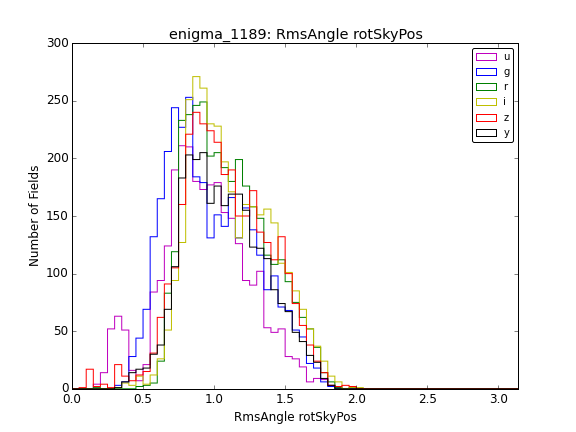
\includegraphics[width=\linewidth]{figs/enigma1189RmsAnglerotSkyPosugrizybandallpropsOPSIComboHistogram.png}
\caption{The relative angle of the detector plane with respect to the sky, RotSkyPos, as a histogram showing the number of fields vs. rms of the parameter.}
\label{RotSkyPos}
\end{figure}

The distribution of rms values by filter is shown in
\autoref{RotSkyPos} for the current candidate baseline simulation,
enigma\_1189.  As shown, the rms values cluster around the value 1
radian,  with typical values 1 +- 0.3 radian.  This compares to a
completely uniform distribution over the half circle with an rms of
1.14.  As mentioned above, uniformity in cosine squared is the goal.
Simulated observing of 100 visits to a field show this will produce
a factor of 10 decrease in CCD-based shear systematics such as edge 
effects and the brighter-fatter x-y anisotropy.

\subsection{Discussion}

The RotSkyPos metric analysis shows that the majority of fields have a
good randomization of detector angles projected on the sky. 

There are some limitations to this observation.

%First, we do not have at present a quantitative requirement for
%randomization of this parameter.  In future development of weak
%lensing analysis, a criterion should be developed.

A significant fraction of fields  have median values that are
lower or higher than expected for a random distribution, with some far
from uniformly distributed.  Regardless of the $per field$ criterion,
it is desirable to avoid the incidence of individual discrepant
fields.

The recommended criterion for randomization of RotSkyPos is not the
behavior of the majority of the fields, but of the minority with the
least random behavior.  The number of non-random fields should be
minimized.  A recommended metric is the count of fields with median
RMS less then 0.8 or greater than 1.5 radians (these values to be
reviewed again as additional experience is gained with additional
OpSim schedule simulations and weak lensing analysis.)

It is certain that actively controlling the statistics of RotSkyPos
will require additional slewing of the camera rotator.  At present,
the operations plan is to only slew when necessary to prepare for a
filter change - that could be estimated at the equivalent of $\simeq
3$ complete rotations per day.  \autoref{RotSkyPos} shows that to
render the distribution completely uniform would require moving all
observing angles an average of $\simeq 30$ degrees, or 300 complete
rotations per night.  The timing of this has not been considered.
Whether or not this uniformity could be achieved with less slew time
if implemented in scheduling remains to be demonstrated.

A similar metric for RotTelPos should be developed.
